\section{Problem Description}
\label{ProbDesc}

We first formally describe a classification task in the supervised learning setting. Then we describe a feedforward neural network with fully connected layers. Feedforward neural networks act as function approximators in such tasks.

\subsection{Classification Problem}
\label{ClassProb}

More formally, given a dataset $ \mathcal{D} = \{x_i,y_i\}_{i=1:N}$ with data points $x_i \in \mathbb{R}^D$ and labels $y_i \in \mathbb{R}^P$, the classification task involves making an accurate label prediction $\hat{y}$ on a previously unseen data point $x$. We approximate the label as a function of the datapoint using a classifier (a feedforward neural network here) with parameters $\theta = \{\theta_k\}_{k=1:K}$ as follows: $y \approx \hat{y} = f(x; \theta)$.
The classifier (neural network) learns the function $f$ from the training data $\mathcal{D}$ by tuning its parameters ($\theta$) to minimize a pre-specified loss function, for instance, the Mean-Squared Error loss:
\begin{align} \label{LMSE}
\mathcal{L}_{MSE} (\theta) = \frac{1}{N}\sum_{i=1}^N ( y_i - f(x_i; \theta))^2
\end{align}

This minimization can be carried out using optimization algorithms like Gradient Descent, Newton's method, Levenberg-Marquardt algorithm etc.
Though Newton's method is a second-order optimization technique, it requires the computation of the hessian of the objective function which is very prohibitive for a large number of parameters like in a neural network.
Levenberg-Marquardt algorithm also requires computing matrices of the size of hessian and can be very slow for classifiers with a large number of parameters.
Currently Gradient Descent is the most successful technique to train huge neural networks with millions of parameters, since it provides a decent tradeoff between convergence speed and memory requirements.
We will describe gradient descent in section \ref{BackProp}.

\subsection{Feedforward Neural Networks}
\label{FNN}

The basic unit of feedforward neural networks is a neuron. A single neuron generally takes a vector of inputs $x \in \mathbb{R}^n$ and outputs a single scalar $a \in \mathbb{R}$ (called its activation). Generally the function computed by a neuron comprises of linear transformation on the input vector followed by a pointwise non-linear activation function:
\begin{align}
a = f(w^T x + b)
\end{align}
where $w \in \mathbb{R}^n$ is called the weight vector and $b \in \mathbb{R}$ is the scalar bias of the neuron.
Many different kinds of activation functions have been studied and used according to the task at hand e.g. linear, sigmoid, tanh, ReLU etc. We will use the sigmoid and linear$(f(z) = z)$ activation functions in our implementation.

\begin{figure}[ht]
%\vskip 0.2in
\begin{center}
\centerline{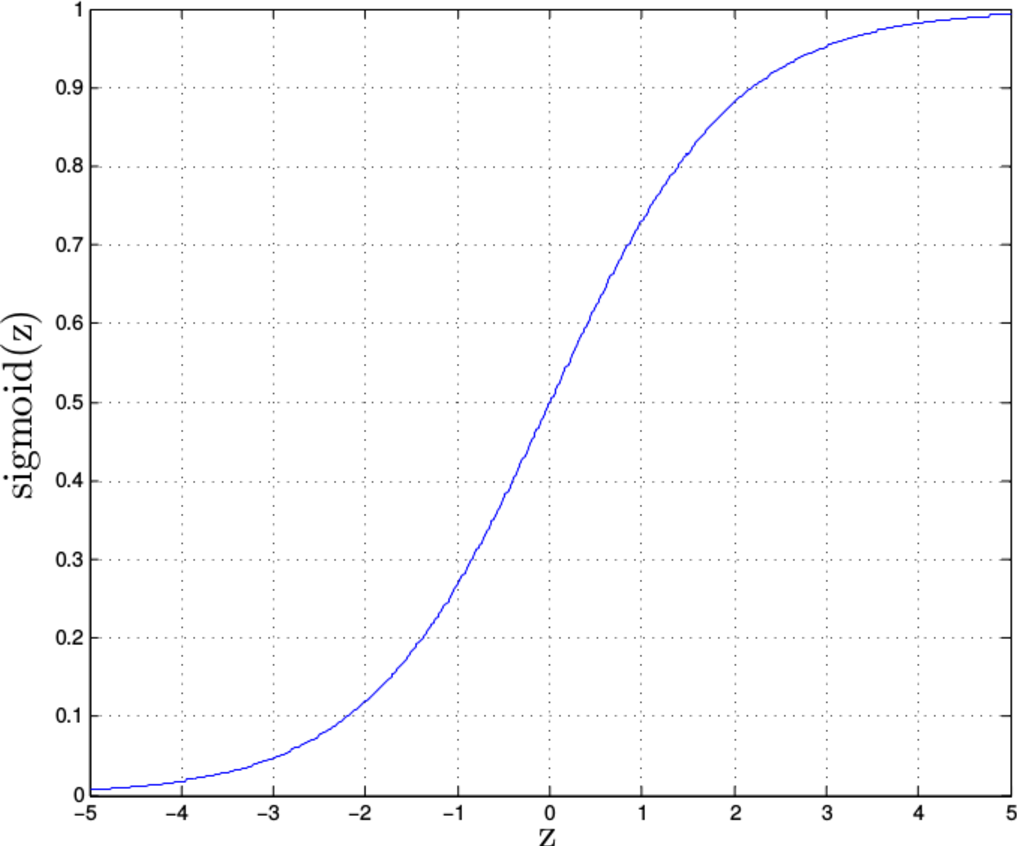
\includegraphics[width=\columnwidth]{sigmoid}}
\caption{The sigmoid function}
\label{fig:sigmoid}
\end{center}
\vskip -0.4in
\end{figure}

The sigmoid function is shown in figure \ref{fig:sigmoid} and is defined as follows:
\begin{align}
f(z) = \frac{1}{1 + e^{-z}}
\end{align}
A feedforward neural network is a directed acyclic graph $G = (V,E)$ each of whose vertices $v \in V$ is a neuron and every edge $(u,v) \in E$ represents the output of neuron $u$ going as an input to neuron $v$. In general to have a more concrete structure the graph $G$ is organized into a layered structure and we will only use layered feedforward neural networks in our implementations. 

A feedforward network with $L$ layers comprises of a single input layer, $L-2$ hidden layers (their outputs are not directly observed) and a final output layer.
Let the input of the neural network be $x \in \mathbb{R}^{n_{in}}$ and the output be $y \in \mathbb{R}^{n_{out}}$.
The $l^{th}$ layer has $n_l$ neurons and the full network has $n = \sum_{l=1}^L n_l$ neurons.

The input to the first layer (denoted $x_1$) is $x$ and the output (activation) of the first layer is denoted $a_1 \in \mathbb{R}^{n_{in}}$. The input layer contains $n_1 = n_{in}$ dummy neurons each of which takes a single scalar input $n_{in}$ and passes it as it is i.e. $a_1 = x_1 = x$.

All subsequent layers $l \in \{2,3,...,L\}$ give an output $a_l \in \mathbb{R}^{n_{l}}$ and take an input $x_l = a_{l-1} \in \mathbb{R}^{n_{l-1}}$. The final network output $y$ is given by $a_L \in \mathbb{R}^{n_L} (n_L = n_{out})$.
Each of these layers applies a linear transformation to its input followed by a pointwise non-linear activation function i.e. for each layer:
\begin{align}
z_l &= (W^l)^T x_l + b_l \\
a_l &= f(z_l)
\end{align}
where $W^l \in \mathbb{R}^{n_{l-1} \times n_l}$ is the weight matrix of the layer and $b_l \in \mathbb{R}^{n_l}$ is the bias vector. The function $f(\cdot)$ is the pointwise activation function which applies to each component of the $z_l$ vector and we will use sigmoid as our activation function for the classification task.
